\chapter{YPC的功能模块}

YPC在可信域和不可信域均有重要的功能和协议设计。本章试图模块化地抽象YPC,找出各组件之间的联系和依赖关系。从这些依赖关系中,找出与TEE各功能的对应关系,进而得出YPC对于TEE的依赖范围。

\begin{figure}
    \centering
    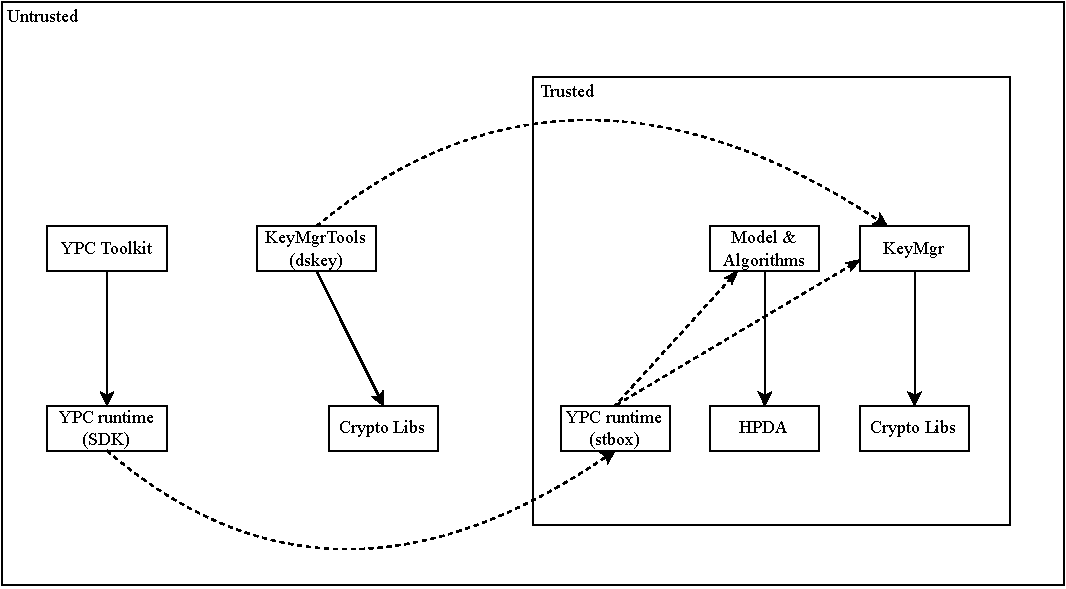
\includegraphics[width=140mm]{figure/ypc-modular.pdf}
    \caption{YPC模块关系图。整个系统分为两个区域,二者信任模型不同:其中Trusted为可信域,在TEE中存储和执行;Untrusted为不可信域,在TEE外执行。两个区域各有YPC运行时(runtimes)用于同步数据和系统状态。}
    \label{fig:ypc-modular}
\end{figure}

图\ref{fig:ypc-modular}展示了YPC的模块化框图。在初始化阶段,运行在非可信域中的KeyMgrTools将由EK加密后的平台相关密钥信息,通过可信信道传输到可信域中的KeyMgr中。

\begin{itemize}
    \item $S^D_c = seal_{EK}(S^D_p)$
    \item $S^D_p = unseal_{EK}(S^D_c)$
\end{itemize}

在YPC中,该功能由KeyMgrTools和KeyMgr共同实现。SGX对于该功能的支持,称作seal/unseal,其信任根是EK。KeyMgr通过seal,将平台相关的密钥信息存储到磁盘上;KeyMgrTools通过unseal,将平台相关的密钥信息传输到KeyMgr中。KeyMgrTools和KeyMgr之间的通信,通过可信信道实现。

在初始化阶段,还需要通过可信认证,验证KeyMgr执行环境的可信性。首先由KeyMgr及TEE平台生成验证报告\texttt{evidence},随后通过互联网连接至远程可信服务器,提交\texttt{(pem-key, evidence)},获得远程可信认证报告。在YPC中,该功能由KeyMgr和Attestation共同实现。SGX对于该功能的支持,称作remote attestation,其本地信任根是EK。

从协议角度,YPC的简化模型包括四个角色,
\begin{enumerate}
    \item 数据提供方(data provider)\\ 
    提供任务图中的原始数据,以自己持有的枢公钥加密原始数据。
    \item (算法)模型提供方(model provider)\\ 
    开发者,算法提供方也可以提供相应的模型。
    \item 数据使用方(data user)\\ 
    得到最终的计算任务输出。
    \item 算力提供方,又称计算平台(computing platform)\\ 
    安装Fidelius隐私计算节点,持有典密钥对$(S^D, P^D)$。
\end{enumerate}

YPC支持的机密计算功能和特性包括,本地数据可用不可见、托管数据可用不可见、结果的可信性证明、结果不可见、数据用途限制、模型不可见、模型用途限制、任务参数不可见、原子交付。

本文描述YPC部分特性的实现方法,并以伪代码形式展示。

\begin{enumerate}
    \item 本地数据可用不可见\\
    由于可信内存(EPC)尺寸有限,本地数据可通过加密后存储到外设上。

    数据提供方通过$P^D$加密数据,并传输到算力提供方:$data_e = \texttt{encrypt}_{P^D}(data)$

    算力提供方在其TEE中解密数据:$data_p = \texttt{decrypt}_{S^D}(data_c)$

    \item 托管数据可用不可见\\
    数据提供方将数据使用自己的公钥$P^S$加密后,托管到第三方存储。在解密时,将数据传输到算力提供方TEE中,通过可信信道私钥转发,获得数据提供方私钥解密数据。

    首先,数据提供方将数据加密:$data_c = \texttt{encrypt}_{P^S}(data_p)$;

    随后,将加密后的数据$data_c$上传到托管平台;

    当需要使用该数据时,将加密数据取回,根据元数据确定数据提供方,在TEE中进行私钥转发,获得$S^S$;
    
    随后,在TEE中通过$S^S$解密数据:$data_p = \texttt{decrypt}_{S^S}(data_c)$。

    \item 结果的可信性证明\\ 
    在初始化阶段,通过可信认证,验证$P^D$的可信性。计算平台得到计算结果后,在TEE内通过$S^D$对结果签名,保证计算结果的正确性完整性。

    $certificate = sign_{S^D}(hash(result))$

    \item 结果不可见\\ 
    计算平台得到计算结果后,在TEE中将结果通过数据使用方公钥$P^S$加密后,返回数据使用方。

    $result_c = encrypt_{P^S}(result_p)$

    \item 数据用途限制\\ 
    (还未实现)计算平台解析元数据,检查数据用途。

%     \begin{lstlisting}
% // Check params in model enclave
%     \end{lstlisting}

    \item 模型不可见\\ 
    模型源代码不可见,仅将编译后的二进制文件传入计算平台,而不显式地公布源代码或模型参数。

    未来可能的实现方法是,将模型通过$P^D$加密后,发送至计算平台。

    $model_c = encrypt_{P^D}(model_p)$

    \item 模型用途限制\\ 
    计算平台解析模型元数据,检查模型参数和用途。

    首先解密模型:$model_p = decrypt_{S^D}(model_c)$。

    如果解密成功,解析模型元数据,检查模型用途。若解密失败(未获取到模型提供方私钥),即模型不可用。

    \item 任务参数不可见\\ 
    数据使用方将计算任务参数加密后,传入计算平台。
    
    $params_c = encrypt_{P^D}(params_p)$
    
    \item 原子交付\\
    通过智能合约(Revocable SC ?),保证任务结果交付和任务费用交付的原子性绑定。

%     \begin{lstlisting}
% // Chains and smart contracts
%     \end{lstlisting}

\end{enumerate}

